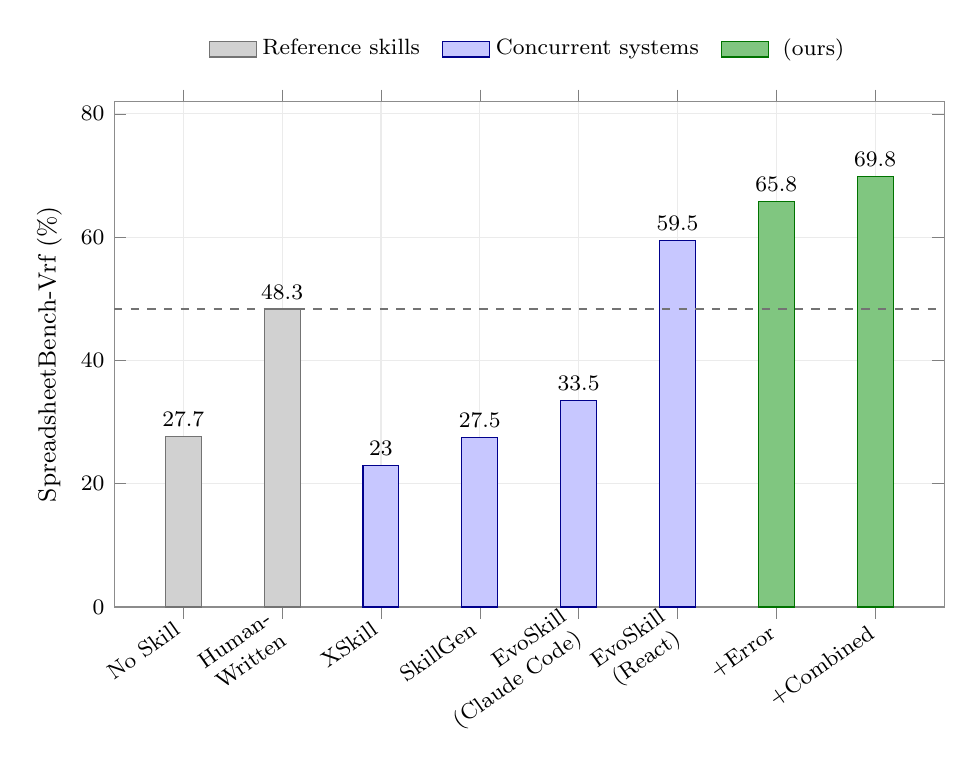
\begin{tikzpicture}
\begin{axis}[
    width=\columnwidth,
    height=0.66\columnwidth,
    ybar,
    bar width=13pt,
    xmin=0.3, xmax=8.7,
    ymin=0, ymax=82,
    ytick={0,20,40,60,80},
    ylabel={SpreadsheetBench-Vrf (\%)},
    xtick={1,2,3,4,5,6,7,8},
    xticklabels={
        No Skill,
        {Human-\\Written},
        XSkill,
        SkillGen,
        {EvoSkill\\(Claude Code)},
        {EvoSkill\\(React)},
        {\systemname{}\\+Error},
        {\systemname{}\\+Combined}
    },
    xticklabel style={font=\footnotesize, rotate=35, anchor=east, align=right, yshift=-1pt},
    yticklabel style={font=\footnotesize},
    ylabel style={font=\small},
    nodes near coords,
    nodes near coords style={font=\footnotesize, /pgf/number format/fixed, /pgf/number format/precision=1},
    every node near coord/.append style={anchor=south},
    grid=major,
    grid style={black!8},
    axis line style={black!45},
    area legend,
    legend style={
        at={(0.5,1.06)}, anchor=south, draw=none, fill=none,
        font=\footnotesize, legend columns=3,
        /tikz/every even column/.append style={column sep=6pt}
    },
]
% reference skills (No Skill floor, Human-Written shared init)
\addplot[ybar, bar shift=0pt, draw=black!55, fill=black!18]
    coordinates {(1,27.67) (2,48.33)};
\addlegendentry{Reference skills}
% concurrent skill-evolution systems (same model + benchmark)
\addplot[ybar, bar shift=0pt, draw=blue!55!black, fill=blue!22]
    coordinates {(3,23.0) (4,27.5) (5,33.5) (6,59.5)};
\addlegendentry{Concurrent systems}
% ours
\addplot[ybar, bar shift=0pt, draw=green!45!black, fill=green!55!black!50]
    coordinates {(7,65.83) (8,69.83)};
\addlegendentry{\systemname{} (ours)}
% Human-Written starting-skill reference line (drawn directly to avoid value labels)
\draw[dashed, thick, black!55] (axis cs:0.3,48.33) -- (axis cs:8.7,48.33);
\end{axis}
\end{tikzpicture}
